%%%%%%%%%%%%%%%%%%%%%%%%%%%%%%%%%%%%%%%%%%%%%%%%%%%%%%%%%%%%%%%%%%%%%
\section{Motivating Example and Background} \label{sect:background}
%%%%%%%%%%%%%%%%%%%%%%%%%%%%%%%%%%%%%%%%%%%%%%%%%%%%%%%%%%%%%%%%%%%%%
This section motivates our work by means of example and reviews the background concepts that form the basis for our discussion in this paper.


%%%%%%%%%%%%%%%%%%%%%%%%%%%%%%%%%%%%%%%%%%%%%%
\subsection{A Brief Overview of Domain-Driven Design (DDD)}
\label{sect:bg-arch} %
%%%%%%%%%%%%%%%%%%%%%%%%%%%%%%%%%%%%%%%%%%%%%%

Domain-driven design (DDD)~\cite{evans_domain-driven_2004} aims to iteratively develop software around a realistic model of the application domain, which on the one hand thoroughly captures the domain requirements. On the other hand, the model is technically feasible for implementation. According to Evans~\cite{evans_domain-driven_2004}, OOPLs such as Java are a natural fit for use with DDD. Booch~\cite{booch_object-oriented_1986} had earlier pointed out domain models in OOPL should be expressive and feasible because of two main points. First, object naturally represents entities that exist in real-world domains. Second, the construct of object used in OOPL is also a basic construct of modeling languages for high-level analysis and design, that conceptualize and realize the domain. This work uses DDD to refer specifically to object-oriented DDD. As explained in~\cite{evans_domain-driven_2004}, within the DDD approach domain model tends to be the heart of software, which is where the complexity lies. Two main features of DDD is that (1)~feasibility, i.e., a domain model should be the code and vice versa, and (2) satisfiability, i.e., the domain model would satisfy the domain requirements that are expressed in a so-called the ubiquitous language~\cite{evans_domain-driven_2004}. This language is defined for stakeholders, including the domain experts and developers, in an iterative and agile process of eliciting the domain requirements. To obtain these two main features of DDD can be seen as one of the main focus of current works on DDD. 

%%%%%%%%%%%%%%%%%%%%%%%%%%%%%%%%%%%%%%%%%%%%%%
\subsection{MOSA: A Module-Based Software Architecture for DDD}
\label{sect:bg-arch} %
%%%%%%%%%%%%%%%%%%%%%%%%%%%%%%%%%%%%%%%%%%%%%%

%\textbf{\textit{MVC architecture.}}
In practical software development, the MVC architecture models are adopted so that the software can have some sort of GUI to assist the development team in constructing it. The main reason for this is rooted in a general understanding (at least up to recently) that software construction can not be fully automated~\cite{fuggetta_software_2014}, due primarily to the human factors that are involved in the development process. %
%MVC is considered in~\cite{calvary_single-user_1997} to be one of several so-called agent-based design architectures, which help make software developed in them inherently modular and thus easier to maintain. 
Software that is designed in MVC consists of three components: model, view, and controller. The internal design of each of the three components is maintained independently with minimum impact on the other two components. Modularity can further be enhanced by applying the architecture at the module's level (\eg, by adopting another agent-based design architecture named PAC~\cite{coutaz_pac:_1987}), thereby creating a hierarchical design architecture in which a software is composed of a hierarchy of software modules. A software \textit{module} (called PAC object in~\cite{coutaz_pac:_1987} and, more generally, agent in~\cite{calvary_single-user_1997}) is a realization of a coherent subset of the software's functions in terms of the architectural components.

To construct DDD software from the domain model requires an architectural model that conforms to the generic layered architecture~\cite{evans_domain-driven_2004, vernon_implementing_2013}. A key requirement of such model is that they position the domain model at the core layer, isolating it from the user interface and other layers. Evans~\cite{evans_domain-driven_2004} suggests that the MVC architecture model~\cite{krasner_description_1988} is one such model. The existing DDD frameworks~\cite{dan_haywood_apache_2013,paniza_learn_2011} support this suggestion by employing some form of MVC architecture in their designs. We observe from all of these works that the user interface plays an important role in presenting a view of the domain model to the stakeholders in such a way that help them to effectively build the domain model. We thus argue that the MVC architecture must be the backbone of any DDD tool that conforms to the DDD's layered architecture. 

Our previous works~\cite{le_tree-based_2015, le_generative_2018} proposed a variant of the MVC architecture for DDD software, called \abbrv{module-based software architecture}{MOSA}. A key feature of this architecture is that it supports the automatic generations of software modules from the domain model and of the software from these modules.
%
A \textbf{MOSA model} consists in a set of MVC-based module classes. 
A \textbf{module class} is an MVC-based structured class~\cite{omg_unified_2015} that represents modules. This class is composed of three components: a domain class (the model), a view class (the view) and a controller class (the controller). The module class becomes the \textit{owner} of the model, view and controller. The view and controller are parameterized classes that are created by binding the template parameters of two library template classes, named \clazz{View} and \clazz{Controller} (\resp), to the domain class.
%
We present in~\cite{le_generative_2018} a technique for semi-automatically generating a module class from the domain class that it owns. Further, the view is designed to reflect the model structure. A set of module classes are used as input for the \jdomainapp~software framework~\cite{le_jdomainapp_2017} to automatically generate software. In this paper, we will assume that a module class is defined for every domain class.

\begin{figure}[ht]
	\centering
	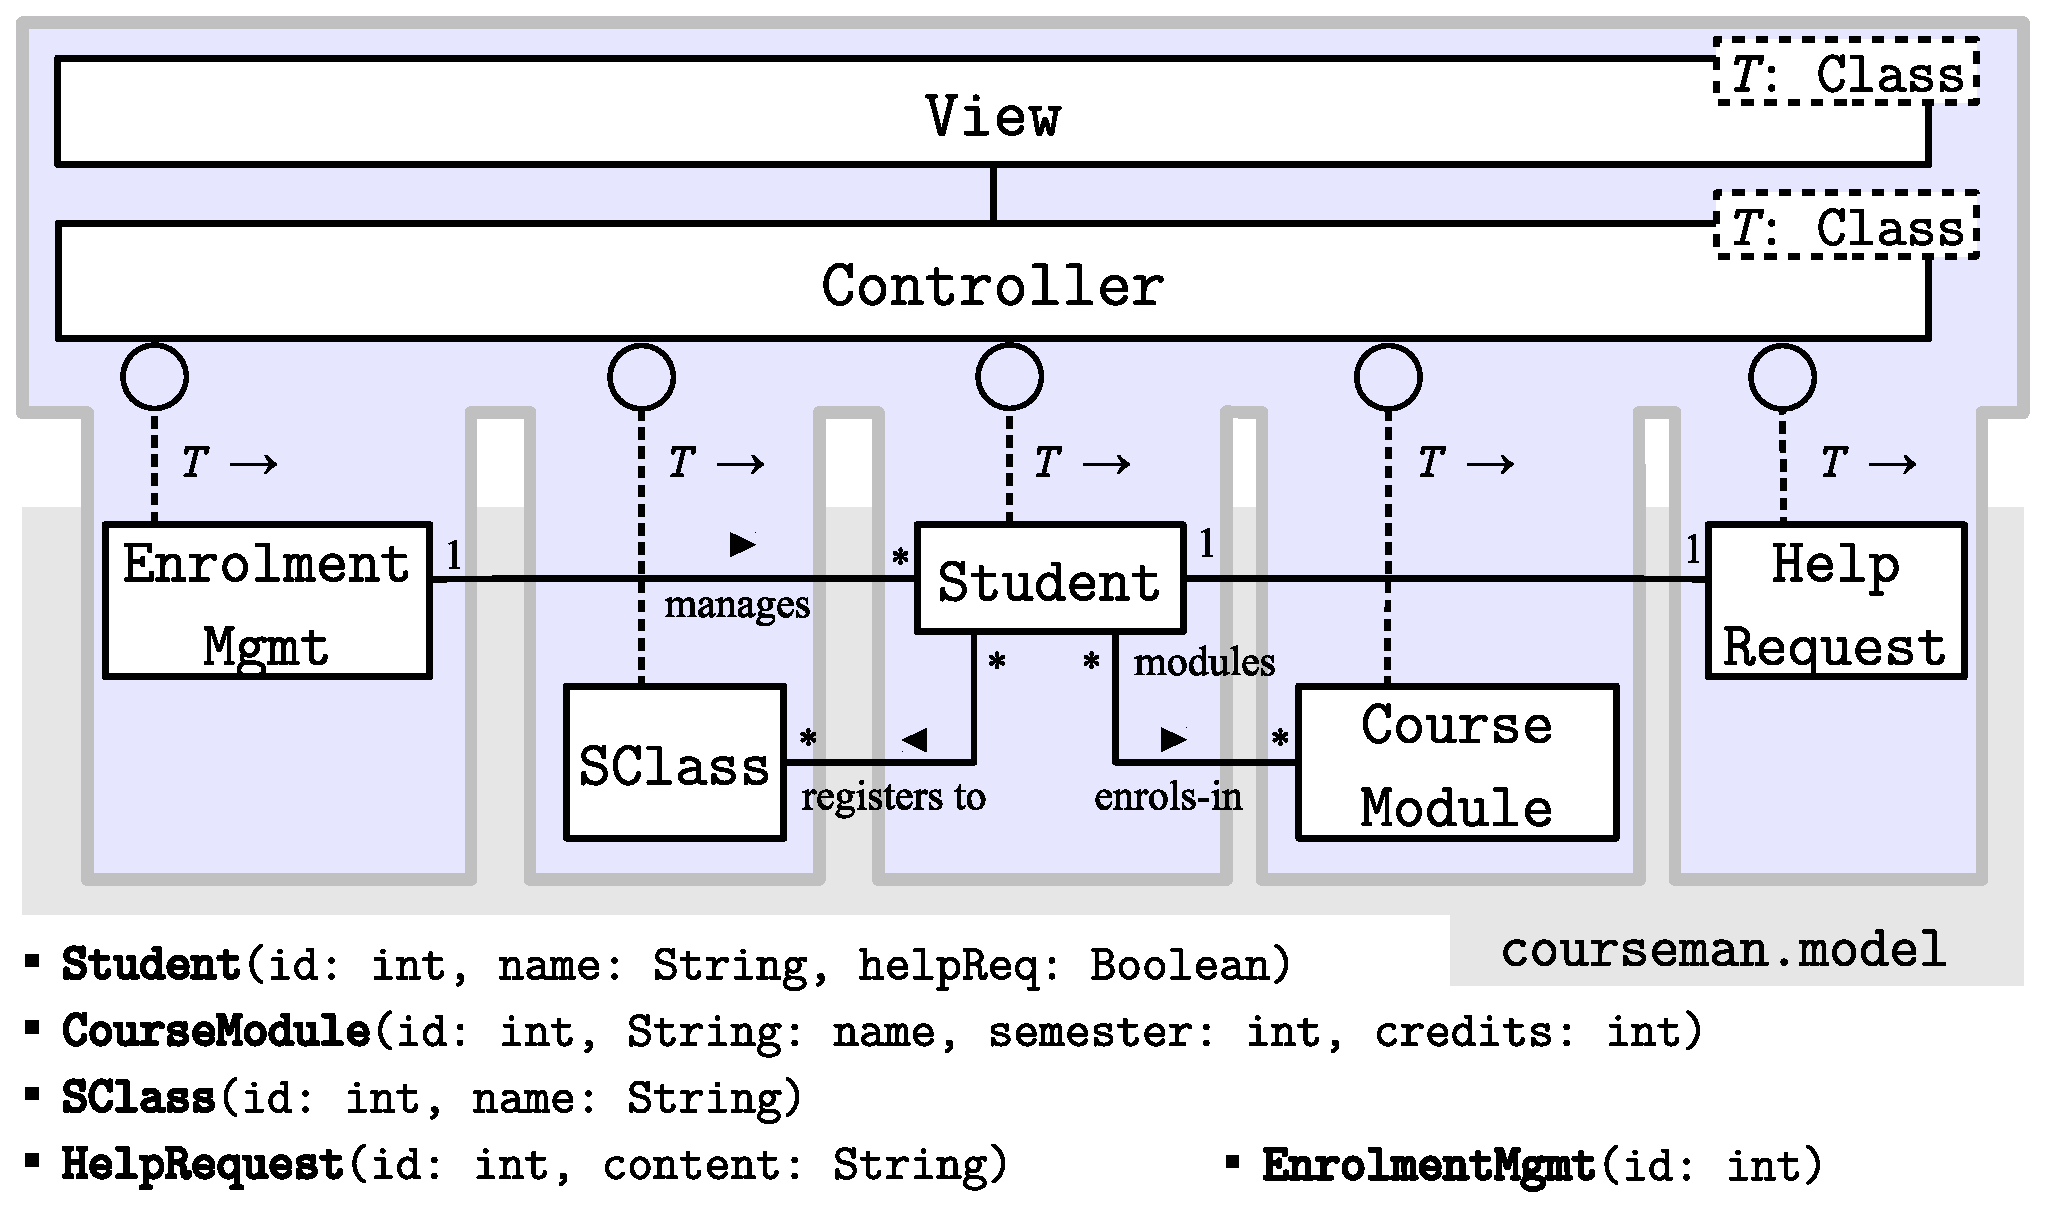
\includegraphics[scale=0.33]{sw-arch/arch-model-courseman}
	\caption{The MOSA model of \courseman.} %
	\label{fig:arch-model-courseman}
\end{figure}

%
To illustrate, the top-half of the MOSA model in Figure~\ref{fig:arch-model-courseman} shows five module classes of \courseman. The parameter bindings are depicted by dashed lines, whose \clazz{Controller}'s and \clazz{View}'s ends are drawn with the symbol `$\bigcirc$'. 
%
%To ease discussion, we name the module classes after their domain classes using the prefix \strq{Module}.
For example, the module class \clazz{ModuleStudent} is composed of three component classes: the domain class is \clazz{Student}, the view is \clazztemplate{View}{\clazz{Student}} and the controller is \clazztemplate{Controller}{\clazz{Student}}.

We argue that MOSA captures the essence of object-oriented software design in a modular, MVC-based design structure. According to Booch~\cite{booch_object-oriented_1986}, an object-oriented software consists of objects and their interactions that are realized though behavior invocation. Given that the domain model is expressed in \dcsl, the MOSA model that has this model at its core helps produce software that possesses the essential behaviors. First, objects are instances of the domain classes in the domain model, which are represented in \dcsl~with the essential structural features. Second, interaction among the objects of a group of domain classes is performed through an event-based message passing mechanism that is managed by the owner modules of these domain classes. This mechanism, which is described in detail in~\cite{le_jdomainapp_2017}, maps events to the essential behaviors that are supported in \dcsl. The events can be triggered by the user interaction on the view of a concerned module. %
%
%However, in~\cite{le_domain_2018} we scoped our use of MOSA at the boundary of the domain model and assumed that this model is connected to the rest of MOSA model via an activity graph. To express this graph in the context of MOSA requires exposing the component interface of the software modules and connecting this interface to the graph. We call this interface the module interface and discuss its design in Section~\ref{sect:actSemantics}. 
%We propose a language for expressing activity graphs in Section~\ref{sect:agl}.

%%%%%%%%%%%%%%%%%%%%%%%%%%%%%%%%%%%%%%%%%%%%%%
\subsection{Representing Domain Models in \dcsl}
\label{sect:bg-dcsl}
%%%%%%%%%%%%%%%%%%%%%%%%%%%%%%%%%%%%%%%%%%%%%%

In the previous work~\cite{le_domain_2018} we have defined an \textit{annotation-based domain specific language}~(aDSL) named \textit{Domain class specification language}~(DCSL) in order to express the domain models. 

\abbrv{Annotation-Based Domain Specific Language}{\textbf{aDSL}} is coined in~\cite{nosal_language_2016} as an attempt to formalise the notion of fragmentary, internal DSL~\cite{fowler_domain-specific_2010} for the use of annotation to define DSLs. An aDSL is defined based on an OOPL's abstract syntax model~\cite{le_domain_2018} that consists of the following meta-concepts: class, field, method, parameter, annotation, and property. These meta-concepts are common to two popular host OOPLs: Java~\cite{gosling_java_2014} and C\#~\cite{hejlsberg_c_2010}. %
%\textbf{\textit{AtOP.}}
Our idea of using annotation to represent modeling rules and constraints is inspired by AtOP \cite{wada_modeling_2005, cepa_representing_2005,sulir_recording_2016,balz_embedding_2012}. In principle, AtOP extends a conventional program with a set of attributes, which capture application- or domain-specific semantics \cite{cepa_representing_2005}. These attributes are represented in contemporary OOPLs as annotations. 
%
We stated in~\cite{le_domain_2018} that using aDSL for DDD brings three important benefits for domain modeling: feasibility, productivity, and understandability. Feasibility comes from the fact the domain model is feasible for implementation in a host OOPL. Productivity is achieved by leveraging the host language platform tools and libraries to process and transform the domain model into other forms suitable for constructing the software. Understandability of the domain model code is enhanced with the introduction of domain-specific annotations.

%Within the scope of this paper and based on the DSL classification in~\cite{kleppe_software_2008}, we differentiate between two types of aDSL: horizontal and vertical aDSLs.
%A \textit{vertical aDSL} targets a bounded real-world (vertical) domain. In contrast, a \textit{horizontal aDSL} (\aka technical aDSL) targets a technical (low-level) domain, whose concepts describe the patterns that often underlie a class of vertical domains that share common features. 
%%Thus, horizontal DSL has a wide scope of application because it is used to build a class of vertical DSLs.
%More specifically, a horizontal aDSL is a DSL internal to a host OOPL, whose domain is a technical one and that uses a set of annotations to model the domain concepts.
%For example, the \courseman's domain model presented in Figure~\ref{fig:arch-model-courseman} can be used as the meta-model for a vertical aDSL for the \courseman~domain. We discussed in~\cite{le_domain_2018} how this domain model is expressed in a horizontal aDSL named \dcsl. A partial \dcsl's domain model of \courseman~is shown in Figure~\ref{fig:dcsl_courseman}. We will review \dcsl~and explain this example in the next subsection.
% In Section~\ref{sect:agl}, we propose another horizontal aDSL for expressing activity graphs. 

\abbrv{Domain class specification language}{\name{DCSL}}~\cite{le_domain_2018} is a horizontal aDSL that we developed to express domain models.
A key feature of \name{DCSL} is that its meta-concepts model the generic domain terms that are composed of the core OOPL meta-concepts and constraints. More specifically, meta-concept \textbf{Domain Class} is composed of meta-concept \clazz{Class} and a constraint captured by an annotation named \clazz{DClass}. This constraint states whether or not the class is mutable. Similarly, meta-concept \textbf{Domain Field} is composed of meta-concept \clazz{Field} with a set of state space constraints. 
These constraints are represented by an annotation named \clazz{DAttr}. 
Meta-concept \textbf{Associative Field} represents Domain Field that realizes one end of an association between two domain classes. \dcsl~supports all three types of association: one-to-one (\abbr one-one), one-to-many (\abbr one-many) and many-to-many (\abbr many-many). 
Finally, meta-concept \textbf{Domain Method} is composed of \clazz{Method} with a commonly-used constraints and behaviour types that are often imposed on instances of these meta-concepts in a domain model. The essential behavior types are represented by an annotation named \clazz{DOpt} and another annotation named \clazz{AttrRef}. The latter references the domain field that is the primary subject of a method's behavior.

%Syntactically, we write a \dcsl~model directly using the host OOPL's syntax. For exposition purposes, however, we write this model using an extended UML graphical notation that uses a \textit{structured text box} for writing annotations. Specifically, non-annotation elements are drawn using the usual UML class diagram notation. On the other hand, the annotation elements are drawn using UML note box. Annotation assignment is represented by a dashed grey line, whose target element end is marked with the attachment symbol (\drawFilledRect[gray]{0.15cm}{0.15cm}). The note box content has the form $ A \; \{ props \} $, where $ A $ is the annotation name and $ props $ is a property listing. Each entry specifies the initialization of a property to a value. 
%%If this value is another annotation element then this element is written using a nested, borderless note box. 
%The entries are separated by either a next line or a comma (`,') character.

%Another feature of the above notation is the use of a virtual (dashed) association line to represent a pair of \clazz{DAssoc} elements that help realise the association ends of an association. This association line is more compact and thus helps significantly ease drawing and improves readability of the model. We will often use the term ``association'' to refer this association line and the \Name{DCSL} model elements that realise it.

\begin{figure}[ht]
	\centering
	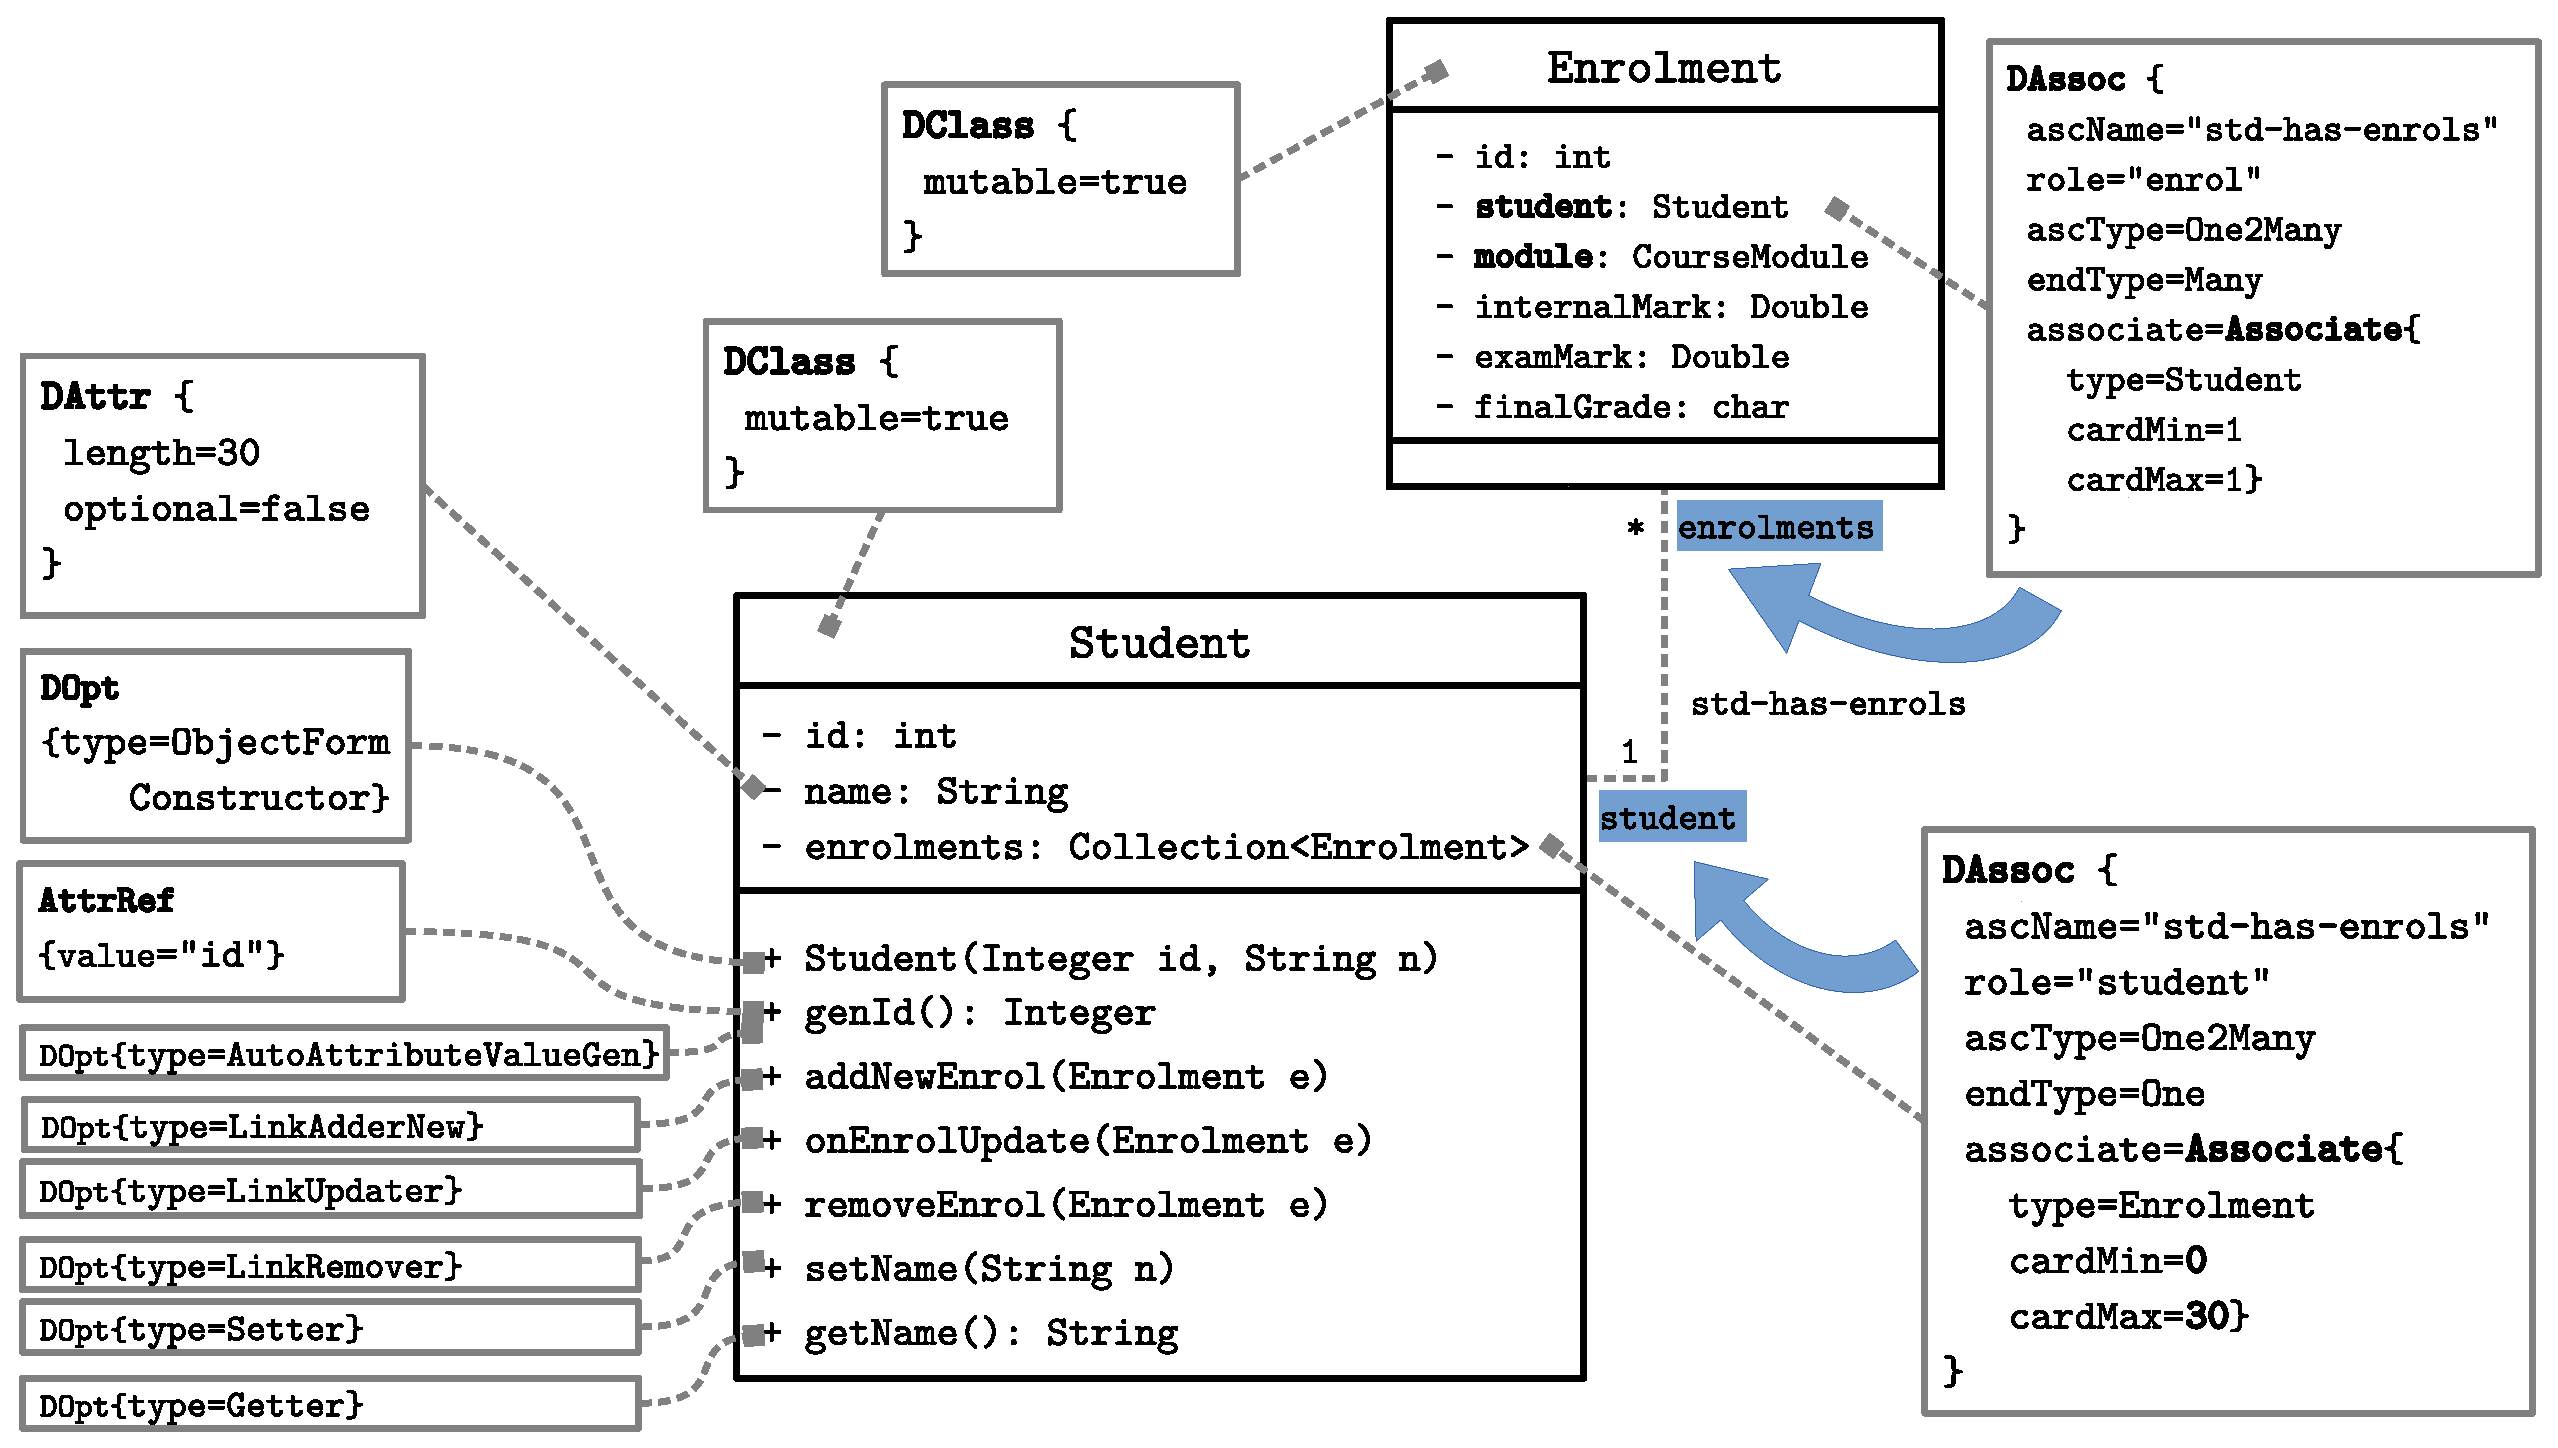
\includegraphics[scale=0.35]{dcsl-model-courseman}
	\caption{A partial \courseman domain model expressed in \dcsl~(adapted from~\cite{le_domain_2018}).}
	\label{fig:dcsl_courseman}
\end{figure}

Figure~\ref{fig:dcsl_courseman} shows a partial \courseman's domain model expressed in \dcsl. This model involves two domain classes: \clazz{Student} and \clazz{Enrolment}. 
%Class \clazz{Enrolment} realises the many-many association between \clazz{Student} and \clazz{Course} (encapsulated by \clazz{CourseModule} as explained in SubSection~\ref{sect:bg-arch}). 
Both of them are assigned with a \clazz{DClass} element, which states that they are mutable domain classes. In particular, class \clazz{Student} has three domain fields: \attribn{id}, \attribn{name}, and \attribn{enrolments}. Domain field \attrib{Student}{name} is illustrated with an \clazz{DAttr} element which states that it is an optional domain field, whose maximum length is 30 (characters). An optional domain field means that the value of this field needs not be initialised when an object is created. Domain field \attrib{Student}{enrolments} is an associative field, which is assigned with a \clazz{DAssoc} element. This element specifies the \clazz{Student}'s end of the association with \clazz{Enrolment}. The opposite end of this association is specified by another \clazz{DAssoc} element that is assigned to the associative field \attrib{Enrolment}{student}. The two thick arrows in the figure map the two \clazz{DAssoc} elements to the two association ends. 
%
The seven methods of class \clazz{Student} listed in the figure are domain methods. Each method is assigned with a \clazz{DOpt} element, which specifies the behavior type. For instance, method \clazz{genId}, whose behavior type is \code{AutoAttributeValueGen}, is additionally assigned with an \clazz{AttrRef} element, which references the name of the domain field \attrib{Student}{id}. This means that \clazz{genId} is the method that automatically generates values for \attrib{Student}{id}.

%%%%%%%%%%%%%%%%%%%%%%%%%%%%%%%%%%%%%%%%%%%%%%%%%%%%%%%%%%%%%%%%%%
\subsection{Motivating Example and Research Questions} 
\label{sect:bg-courseman-eg}
%%%%%%%%%%%%%%%%%%%%%%%%%%%%%%%%%%%%%%%%%%%%%%%%%%%%%%%%%%%%%%%%%%

% ducmle: OLD
%\begin{figure*}[ht]
%	\begin{center}
%		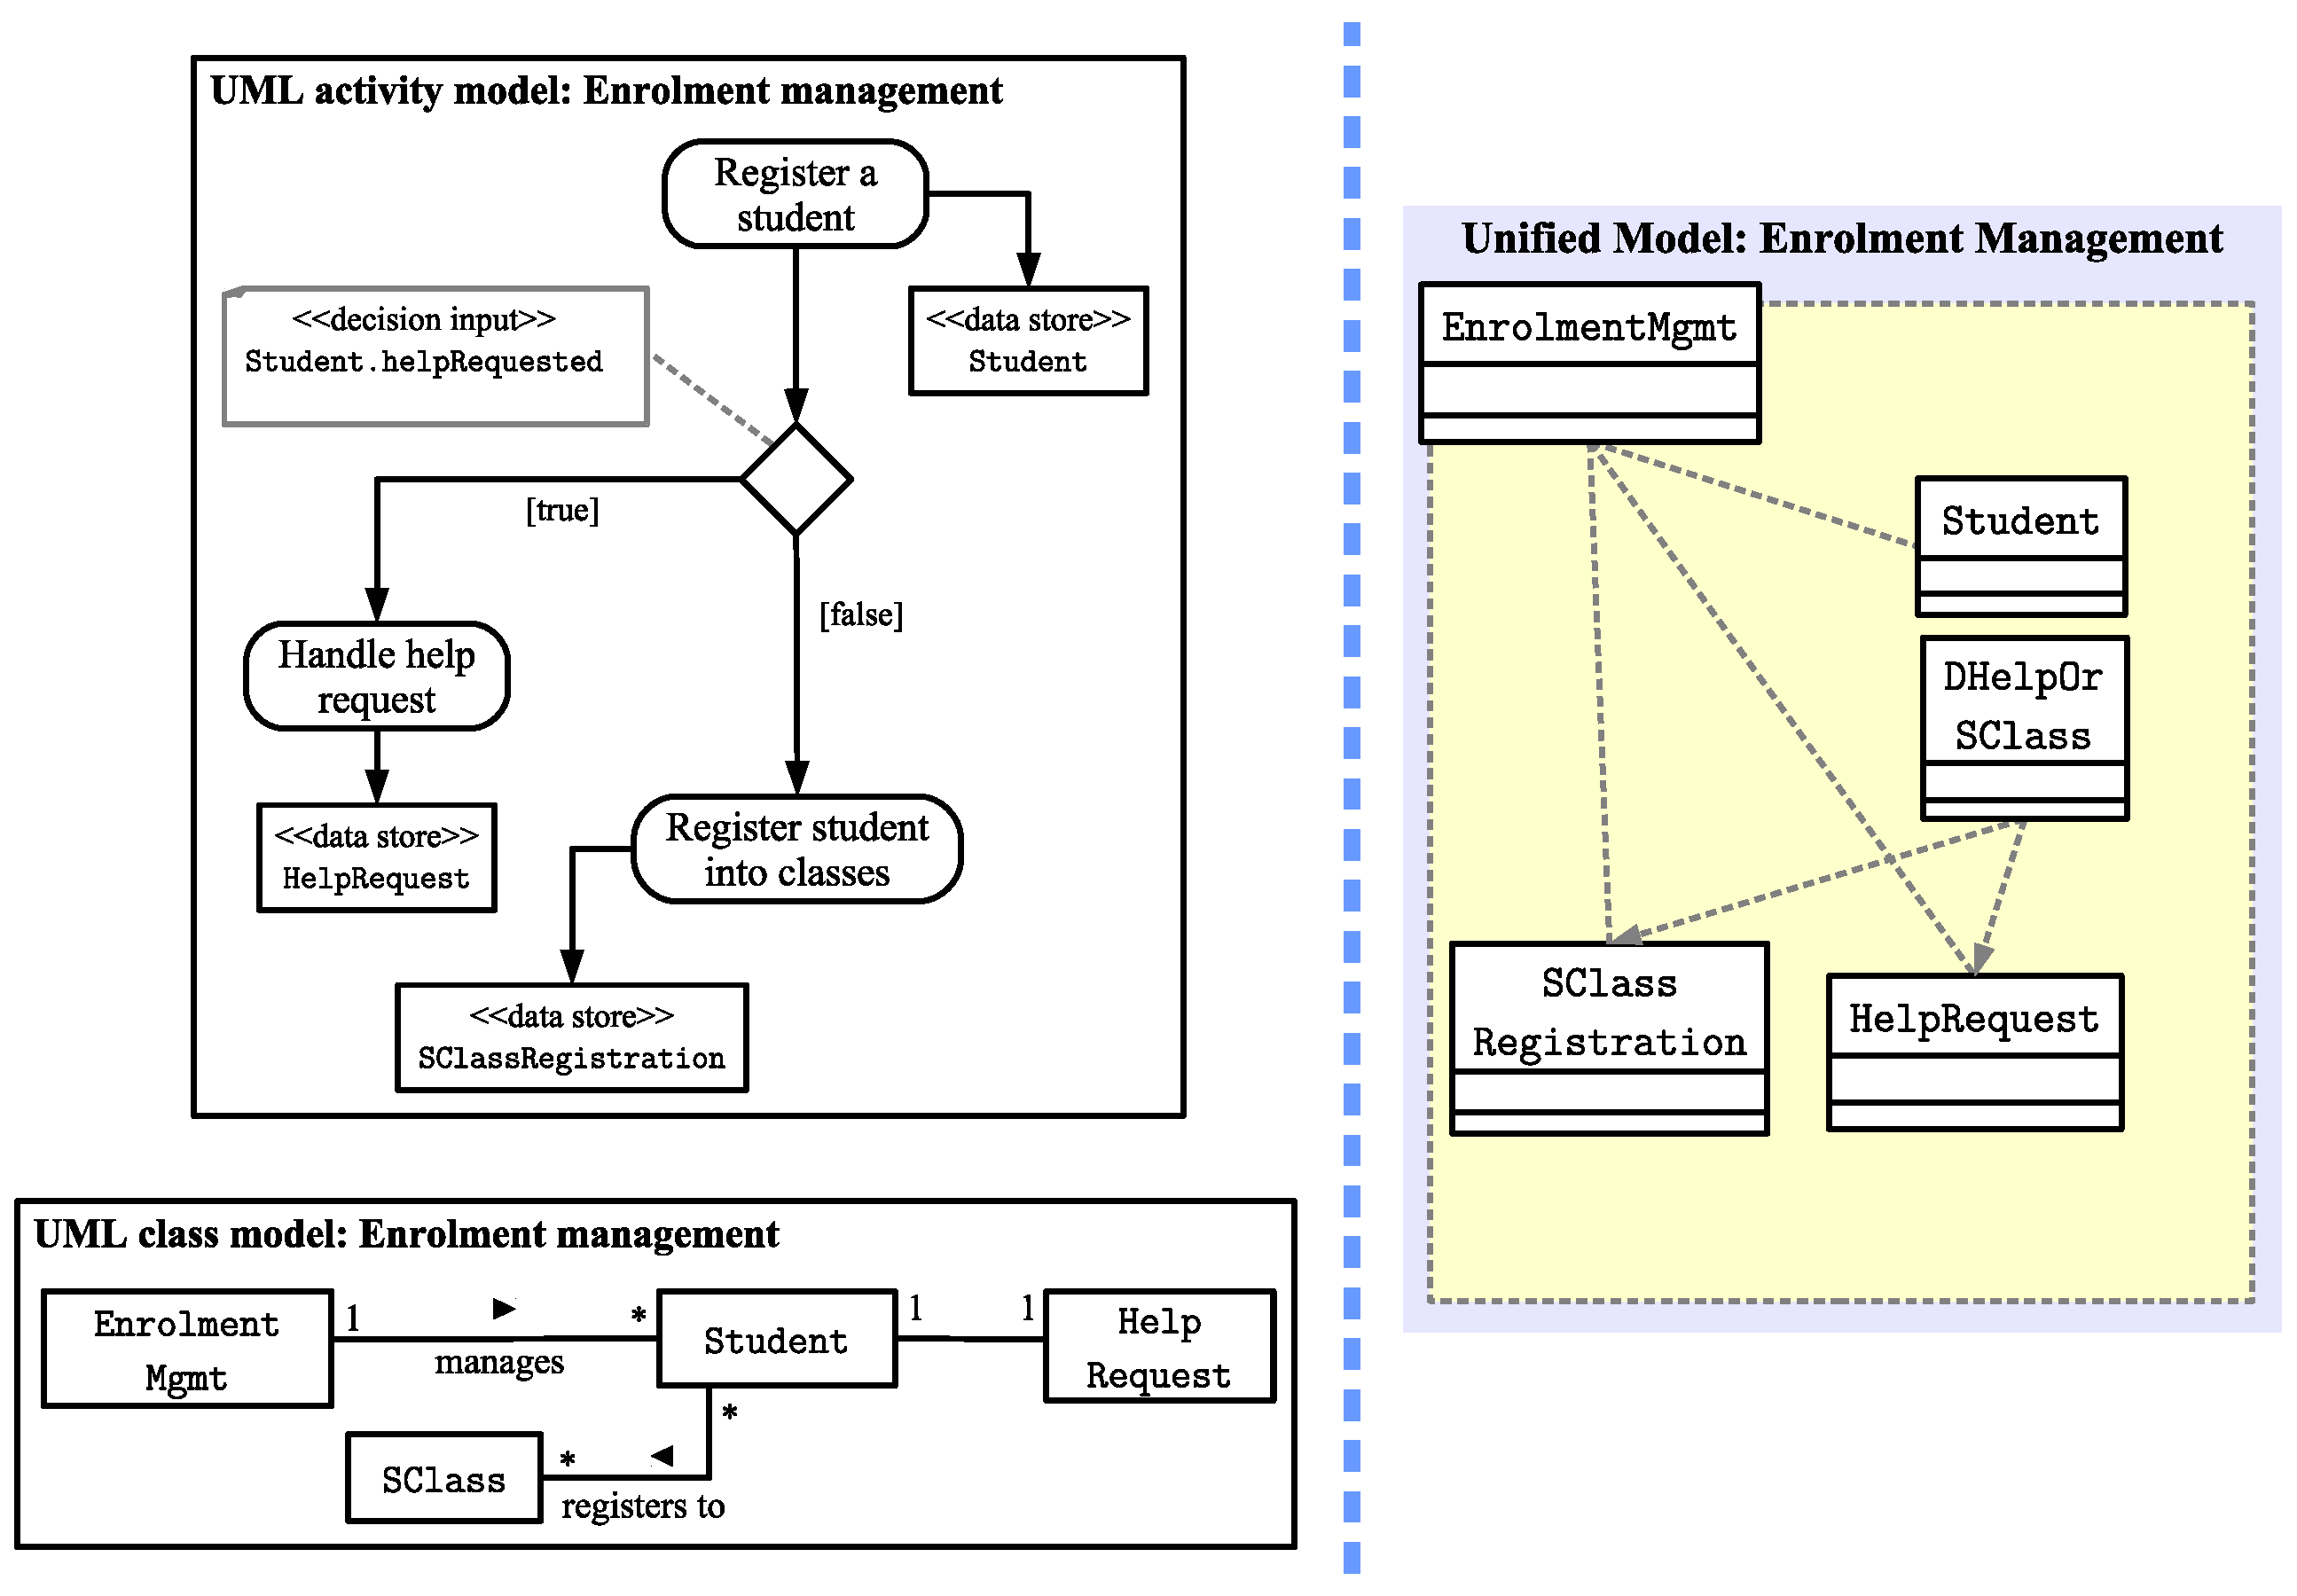
\includegraphics[scale=0.28]{motivatingExample}
%	\end{center}
%	\caption{Simplified UML/OCL class and activity diagrams to specify a \courseman software variant that handles the enrolment management activity.} %
%	\label{fig:motivatingExample}
%\end{figure*} 
We adapt a compact and essential software domain from a previous work~\cite{le_domain_2018}, named course management domain (\courseman) as our motivating example. We introduce here the basic \courseman requirements and use it to illustrate the background concepts. 
%In the rest of the paper, we will use this example and, where necessary, some extensions of it to illustrate our proposed method.

\begin{figure}[th]
\begin{center}
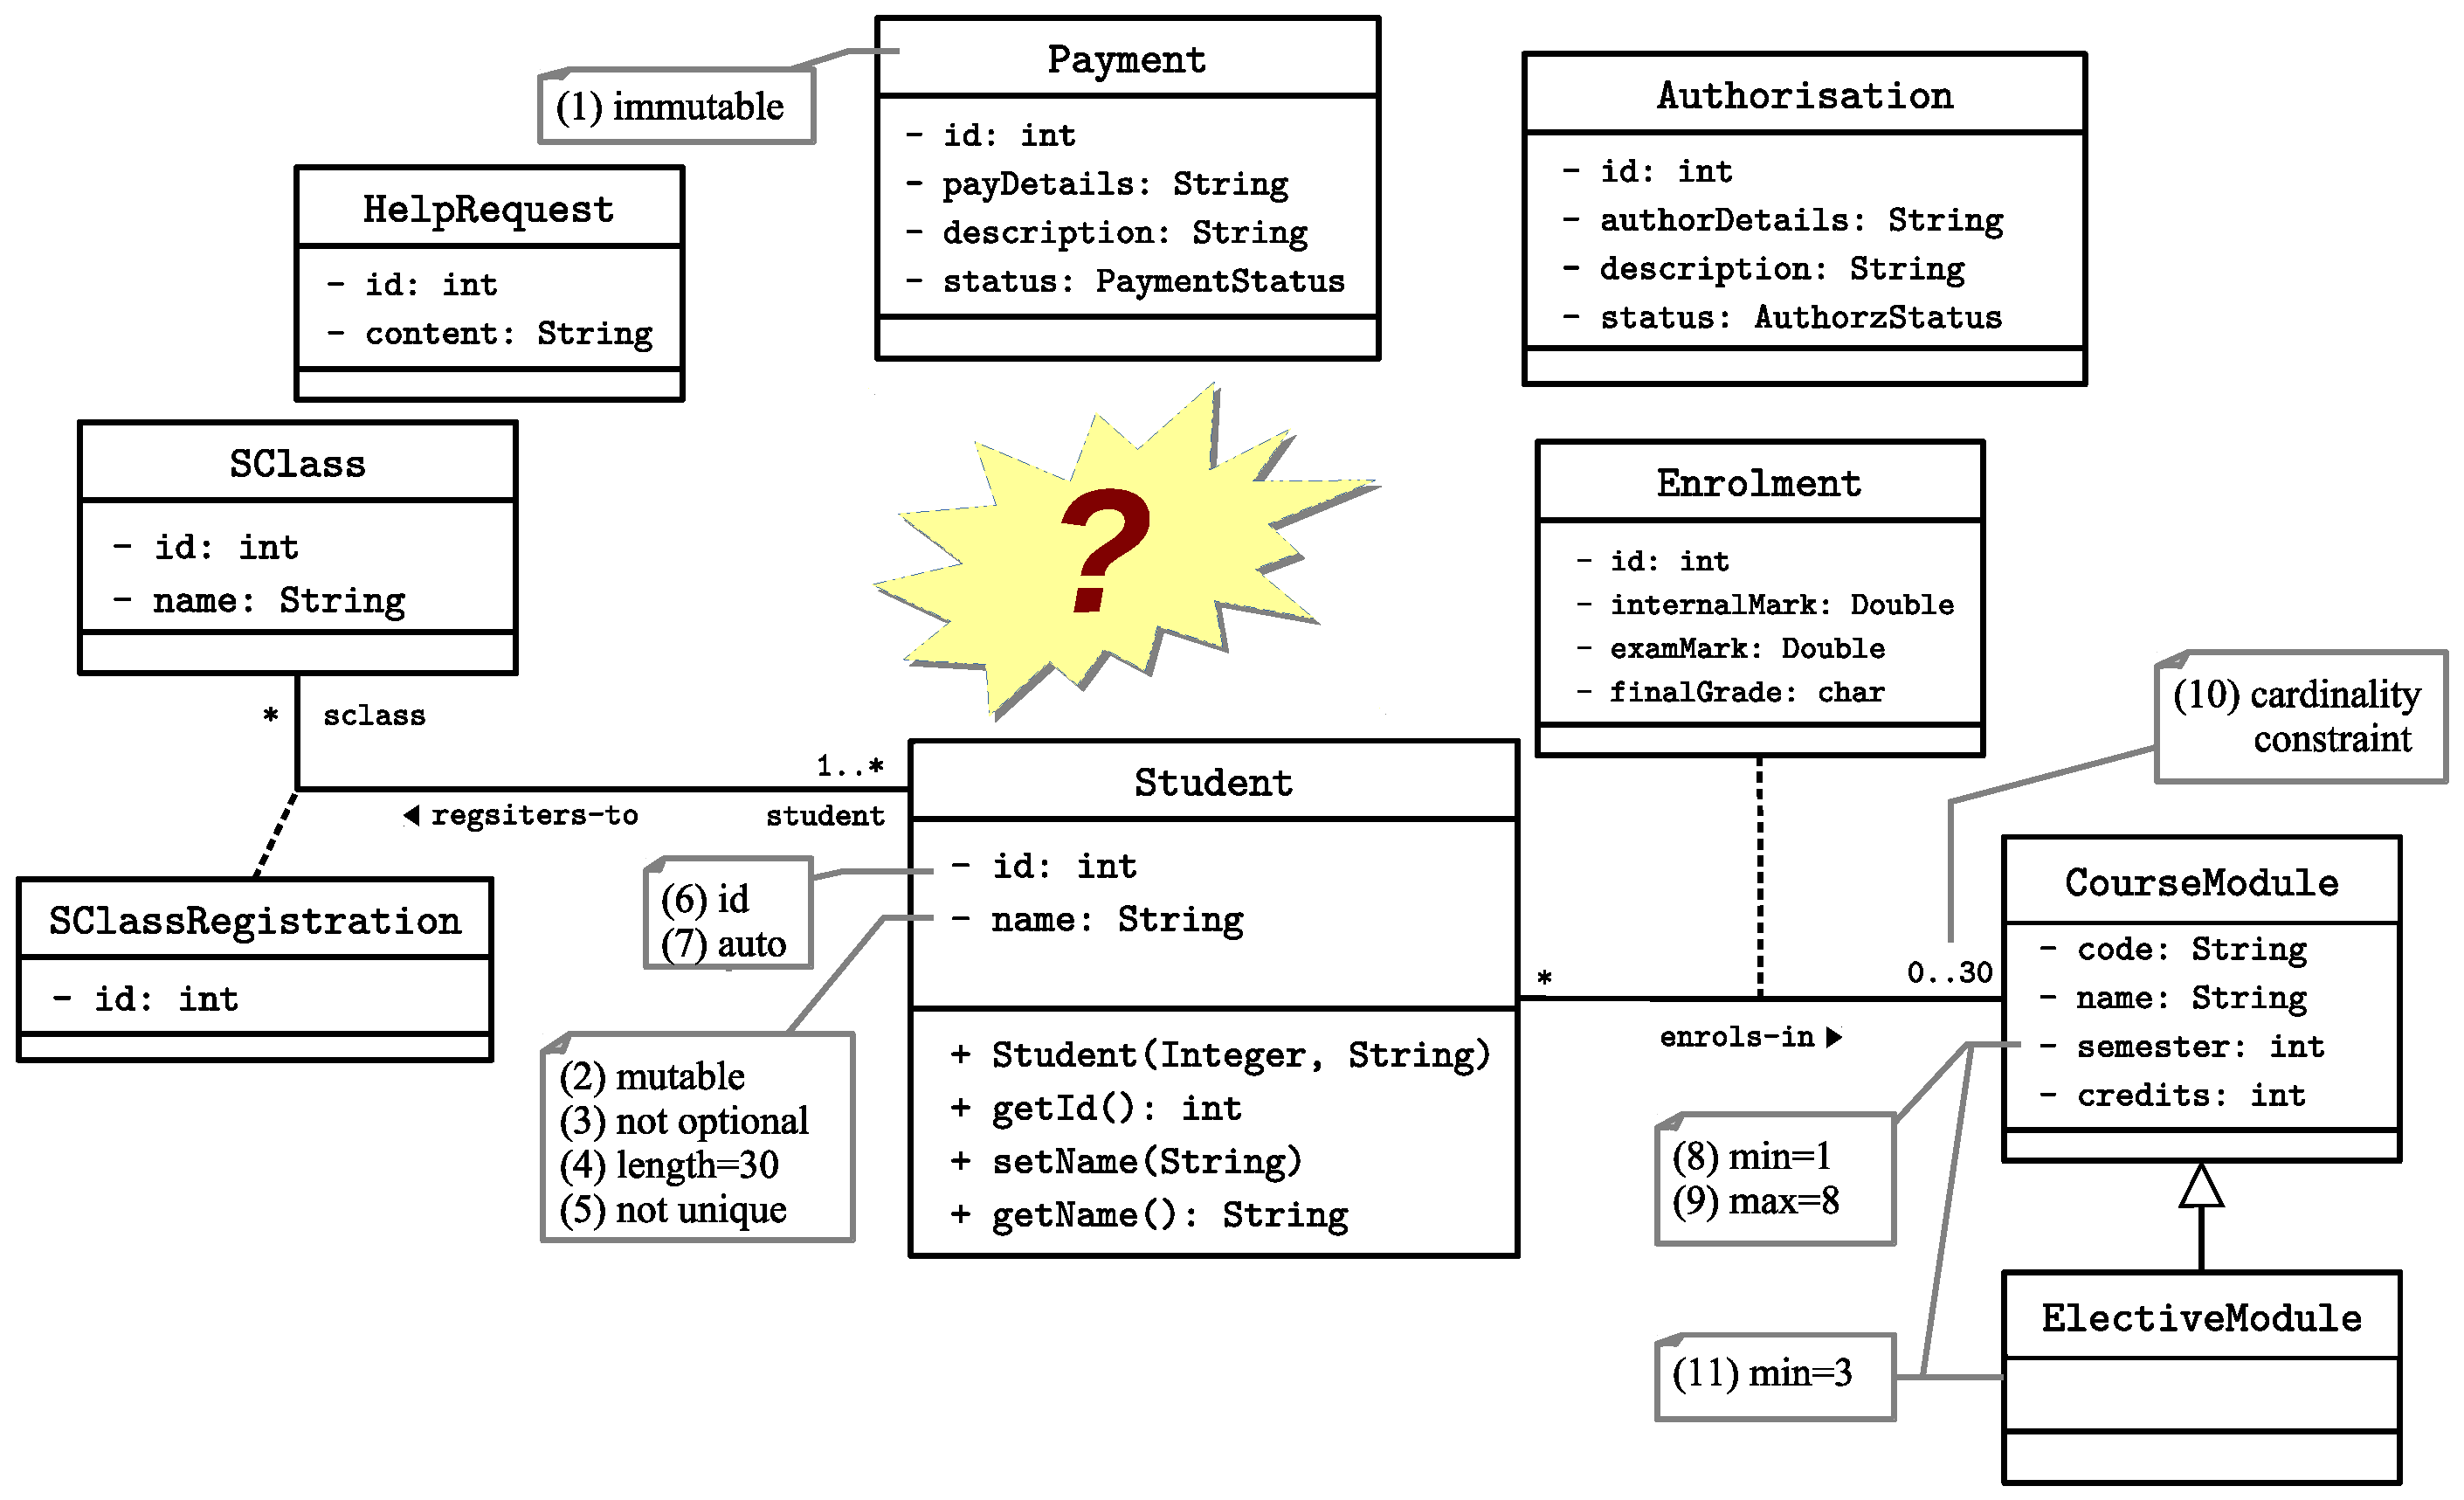
\includegraphics[scale=0.18]{motivating-example}
\end{center}
\caption{The essential domain model of \courseman.}
\label{fig:motivatingExample}
\end{figure}

Figure~\ref{fig:motivatingExample} shows an essential domain model for \Name{CourseMan}, that is represented by a UML class diagram together with OCL constraints. Within our DDD approach~\cite{le_domain_2018} this domain model would be represented in \dcsl. As shown in the bottom part of the figure, this domain model includes four main classes and two association classes: Class \clazz{Student} represents students that register to study in an academic institution; Class \clazz{CourseModule} represents the course modules that are offered by the institution; Class \clazz{ElectiveModule} represents a specialized type of \clazz{CourseModule}; Class \clazz{SClass} represents the student class type for students to choose; Association class \clazz{\clazz{SClass}Registration} captures details about the many-many association between \clazz{Student} and \clazz{SClass}; and association class \clazz{Enrolment} captures details about the many-many association between \clazz{Student} and \clazz{CourseModule}.
As shown in the top part of the figure (with a star-like shape labeled ``?''), this domain model includes also three other classes captured for an enrolment management activity: 
%Suppose that we know some design details (the attributes shown in the figure) and the following description about these classes:
%
\begin{itemize}[noitemsep]
  \item \clazz{HelpRequest}: captures data about help information provided to students.
  \item \clazz{Payment}: captures data about payment for the intuition fee that a student needs to make.
  \item \clazz{Authorisation}: captures data about the decision made by an enrolment officer concerning whether or not to allow a student to undertake the registered course modules.
  % paragraph break
  %\\
\end{itemize}

%We illustrate below how a number of common invariant constraints on \clazz{Student} and \clazz{CourseModule} are expressed in OCL \cite{omg_object_2014}. Other constraints are expressed using more complex OCL expressions and techniques, whose details (see \cite{le_domain_2018}) are beyond the scope of this paper.

%%
%\begin{lstrulex}
%context (@\hterm{Student inv}@):
%  -- constraint (@\hterm{(3)}@):
%  not(name.oclIsUndefined()) and 
%  -- constraint (@\hterm{(4)}@):
%  name.size() <= 30
%
%context (@\hterm{CourseModule inv}@):
%  -- constraint (@\hterm{(8)}@):
%  semester >= 1 and 
%  -- constraint (@\hterm{(9)}@):
%  semester <= 8
%\end{lstrulex}

\begin{figure}[th]
	\begin{center}
		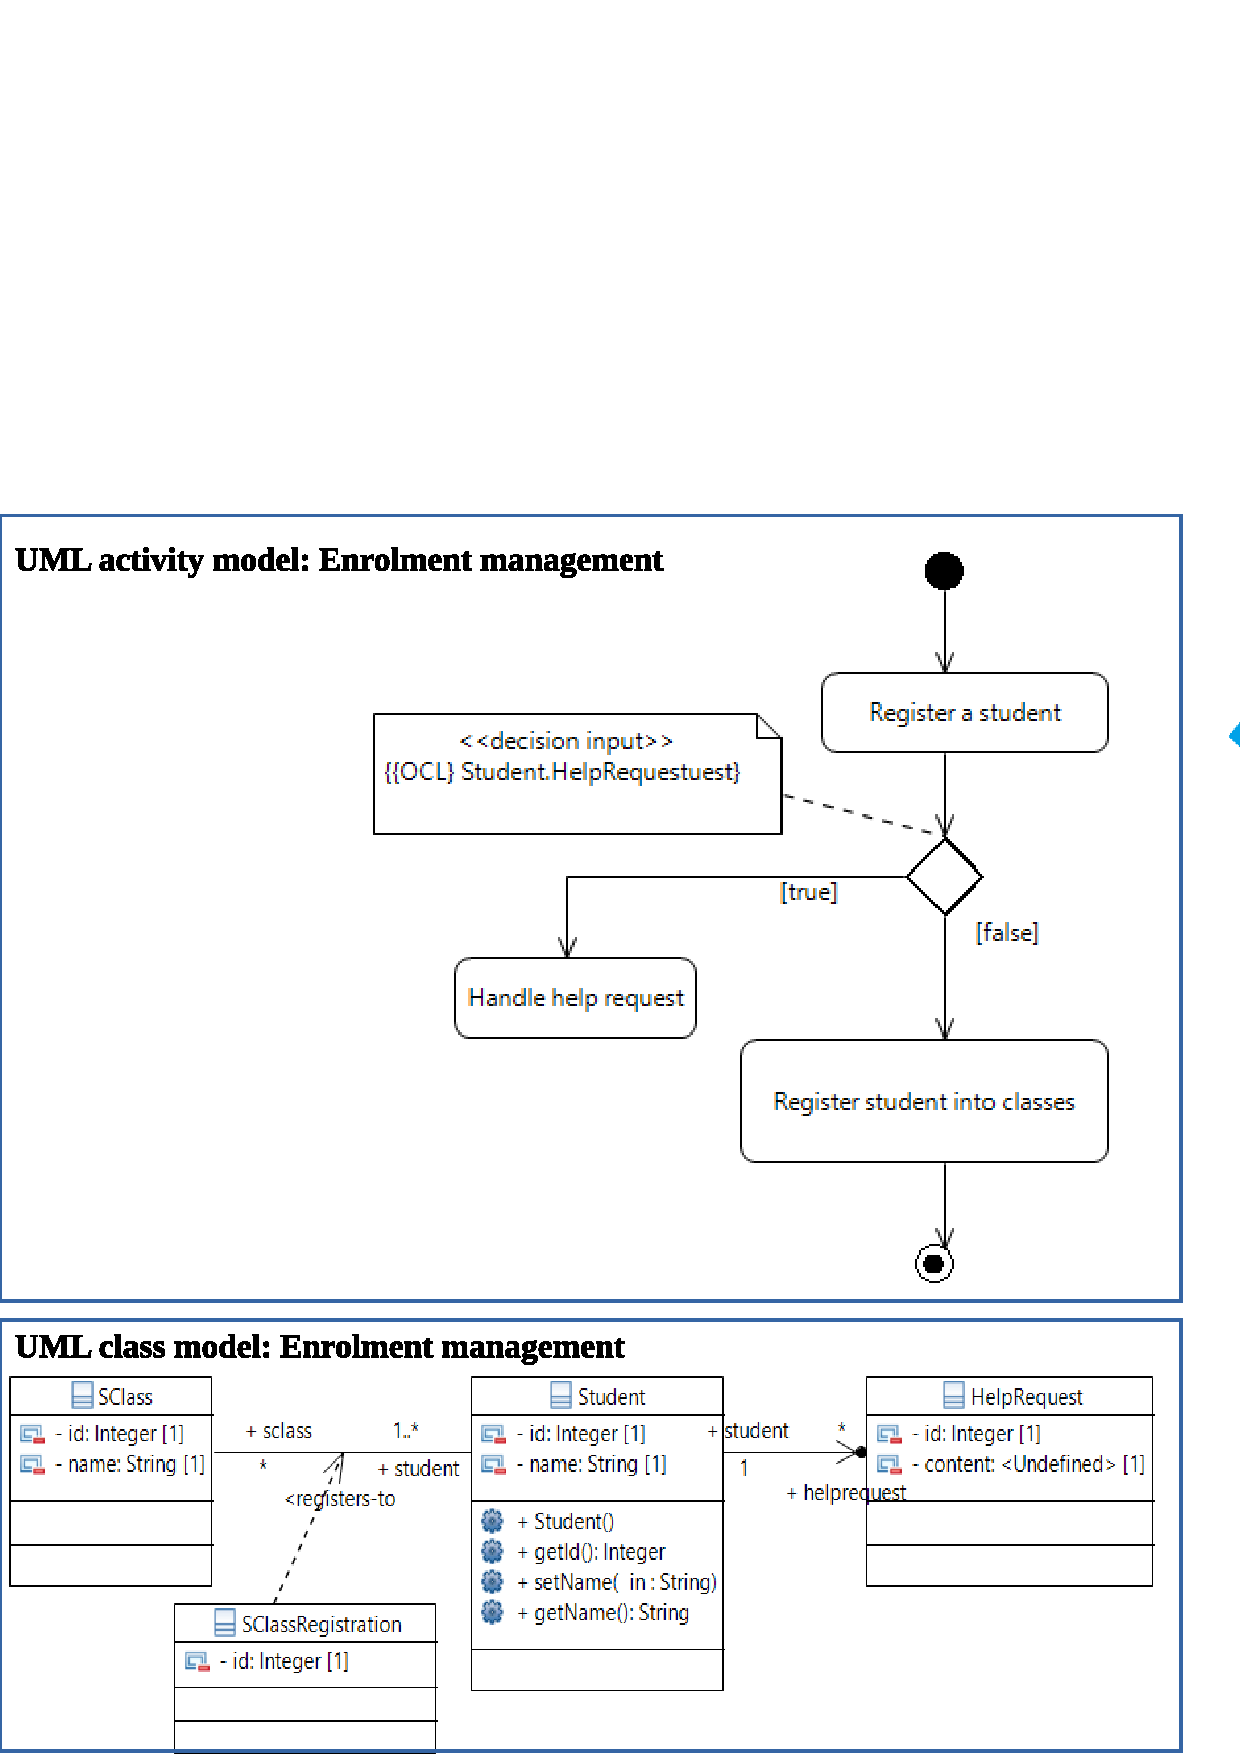
\includegraphics[scale=0.7]{motivating-example2}
	\end{center}
	\caption{A UML Activity diagram to represent the enrolment management activity.}
	\label{fig:motivatingExample2}
\end{figure}

Figure~\ref{fig:motivatingExample2} shows a UML Activity diagram for the enrolment management activity. This activity involves registering \clazz{Student}s, enrolling them into \clazz{CourseModule}s and registering them into \clazz{SClass}es. In addition, it would allow a \clazz{Student} to raise a \clazz{HelpRequest} during the enrolment process. %
%
We might consider the domain behavior as a new concern that needs to be composed with the essential domain model, as shown in Figure~\ref{fig:motivatingExample}, for an executable version of the software. Since this domain behavior is currently captured in UML, we would need a further mechanism to maintain a consistency between the two models, toward composing them, normally at an implementation level. As an alternative approach for this aim, following the DDD approach introduced in our previous work~\cite{le_domain_2018}, we would consider such a behavior concern as an extension of the essential domain model for a unified domain model (i.e., a DDD with the key features, feasibility, productivity, and understandability as explained above). To achieve the goal we face two main challenges that motivates this work as follows:

\begin{enumerate}
    \item How can we extend the DCSL framework (that defines domain models within MOSA for DDD software) with new constructs to represent domain behaviors that could be captured by a UML Activity diagram?    
    \item How can we incorporate such domain behaviors into a DCSL-specified domain model? This would require defining an integrated semantics of structural and behavioral aspects of the domain model.
\end{enumerate}